\section{Ablation}
\label{sec:ablation}

The protocol has four components that a different choice could replace, and each earns its place only if removing it changes a result.
\Cref{tab:ablation} summarises what each removal changes, with the numbers of the experiments of \cref{sec:experimental-design}; the four subsections give the evidence.

\begin{table}[htbp]
\centering
\footnotesize
\caption{Ablation of the protocol: the component removed, what replaces it, the measure on which the two are compared, and its value with and without the component, from the exact coverage calculation, the committed counts, the fifty-block replication and the exact calculations of the instrument experiment.}
\label{tab:ablation}
\fitwidth{\begin{tabular}{p{2.4cm}p{2.5cm}p{4.6cm}p{2.2cm}p{2.2cm}}
\toprule
Component & Replaced by & Measure & With & Without \\
\midrule
Wilson interval & normal approximation & coverage of the 95\,\% interval at a true rate of 0.1\,\% in 4,000 repetitions & \covWilsonThousandth\,\% & \covWaldThousandth\,\% \\
Wilson interval & normal approximation & exact values inside the interval, of \nExactNondeg{} comparisons & \ivWilsonNd{} & \ivWaldNd{} \\
Wilson interval & normal approximation & upper limit for a rate of 0 in 4,000 repetitions (the concentration test) & \hhiWilsonHi\,\% & 0\,\% \\
Screen and definition & rate above the level & share of cells flagged, tests within the level, 4,000 repetitions & \flWithinBoundFour\,\% (screen), \flWithinIntFour\,\% (definition) & \flWithinNaiveFour\,\% \\
Screen and definition & rate above the level & share of cells flagged, tests above the level, 4,000 repetitions & \flOverBoundFour\,\% (screen), \flOverIntFour\,\% (definition) & \flOverNaiveFour\,\% \\
Exact value beside the rate & simulation alone & probability of detecting a generator whose PD is 5\,\% too high & \agFailFivePercent\,\% & none \\
Exact value beside the rate & simulation alone & Jeffreys test at 1\,\%: excess over the level seen by one cell & decided (\jeffExactOne\,\%) & \jeffDetect\,\% \\
4,000 repetitions & 1,000 & excess over 5\,\% seen with probability 0.8 (points) & \detFiveFour & \detFiveThousand \\
4,000 repetitions & 20,000 & excess over 5\,\% seen with probability 0.8 (points) & \detFiveFour & \detFiveTwentyK \\
\bottomrule
\end{tabular}}
\end{table}

\subsection{The interval of a rate}
\label{sec:ab-interval}

\Cref{tab:interval-coverage} and \cref{fig:interval-coverage} give the exact coverage of five nominal 95\,\% intervals for a rejection rate measured in 4,000 repetitions.
Above a true rate of 1\,\% the intervals differ by about one point of coverage at most: at 5\,\% the Wilson, Agresti--Coull and Clopper--Pearson intervals cover \covWilsonFive\,\%, the Jeffreys interval \covJefFive\,\% and the normal approximation \covWaldFive\,\%.
Below it they separate.
At a true rate of 0.1\,\%, where the size of a conservative test sits, the normal approximation covers \covWaldThousandth\,\%, the Wilson interval \covWilsonThousandth\,\%, the Clopper--Pearson and Jeffreys intervals \covCPThousandth\,\% and the Agresti--Coull interval \covACThousandth\,\%, so that the poor coverage of the normal approximation at small proportions that \citet{brown2001} describe is reproduced at the rates of this measurement.
On the committed rows that carry an exact value, the five intervals contain the exact probability in \ivWaldNd{} to \ivWilsonNd{} of the \nExactNondeg{} comparisons that are not at the edge of the unit interval, against the \nExactNondeg{} times 0.95 that nominal coverage would give; the shortfall is small, consistent with the spread of $z$ above one, and it does not separate the methods.
Over all \nExactCmp{} comparisons, including those whose exact value is at the edge of the unit interval, the Wilson, Jeffreys, Agresti--Coull and Clopper--Pearson intervals contain the exact value in \ivWilsonAll{}, \ivJefAll{}, \ivACAll{} and \ivCPAll{}, and the normal approximation in \ivWaldAll{}, because its interval has zero width at a rate of 0 or 1 and so excludes an exact value that is not exactly 0 or 1.
The practical difference is at a rate of zero.
The concentration test rejects in none of 4,000 repetitions, and the normal-approximation interval of that result has zero width, a claim of no uncertainty, while the Wilson interval has an upper limit of \hhiWilsonHi\,\%.
The Wilson interval is therefore adequate everywhere the measurement needs it, and necessary only for the conservative tests; the choice among the score, exact and Jeffreys intervals changes no judgement.

\begin{table}[htbp]
\centering
\footnotesize
\caption{Exact coverage, in percent, of five nominal 95\% intervals for a rejection rate measured in 4,000 repetitions, at five true rejection probabilities, and the number of the committed exact rejection probabilities that fall inside the interval of the simulated rate.}
\label{tab:interval-coverage}
\fitwidth{\begin{tabular}{lrrrrrcc}
\toprule
Interval & $r=0.1$\% & 0.5\% & 1\% & 5\% & 50\% & Exact value inside (63) & Inside (all 94) \\
\midrule
Wald & 90.6 & 94.8 & 94.4 & 94.9 & 94.8 & 56 of 63 & 68 of 94 \\
Wilson & 93.1 & 94.5 & 95.4 & 95.4 & 94.8 & 57 of 63 & 87 of 94 \\
Agresti--Coull & 97.9 & 94.5 & 95.4 & 95.4 & 94.8 & 57 of 63 & 88 of 94 \\
Clopper--Pearson & 96.0 & 95.7 & 96.2 & 95.4 & 95.2 & 57 of 63 & 88 of 94 \\
Jeffreys & 96.0 & 95.7 & 94.4 & 95.0 & 94.8 & 56 of 63 & 87 of 94 \\
\bottomrule
\end{tabular}}
\end{table}


\begin{figure}[htbp]
\centering
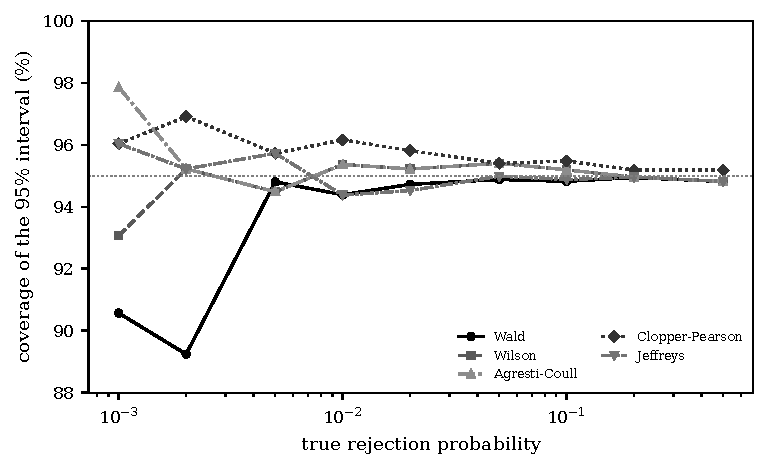
\includegraphics[width=0.85\linewidth]{interval_coverage}
\caption{Exact coverage of five nominal 95\% intervals for a rejection rate measured in 4,000 repetitions, against the true rejection probability on a logarithmic axis: the normal approximation falls well below the nominal coverage at small rates, and the Wilson, Agresti--Coull, Clopper--Pearson and Jeffreys intervals stay near it.}
\label{fig:interval-coverage}
\end{figure}

\subsection{The rule that judges a size}
\label{sec:ab-bound}

The one-sided bound of \eqref{eq:bound}, the screen, and the interval of the definition are compared with the rule that a rate above the level is oversized, on the fifty blocks of every test, grouped by the pooled size of the test (\cref{tab:resolution} and \cref{fig:resolution}).
The group within the level holds conservative tests, whose rate falls away from the level as the cells grow, and tests whose size equals the level, which exceed it in about half of their cells whatever the number of repetitions.
Among the \nWithin{} tests whose pooled size is within the level, the naive rule flags \flWithinNaiveFour\,\% of the cells of 4,000 repetitions, \flWithinNaiveThousand\,\% of the cells of 1,000 and \flWithinNaiveTwentyK\,\% of those of 20,000; the share falls with the repetitions because the conservative tests stop exceeding their level, and it would stay at one half for tests at the level.
The screen flags \flWithinBoundFour\,\% at 4,000 and \flWithinBoundThousand\,\% at 1,000, which is the false flag probability of \cref{prop:false-flag}, and the definition flags \flWithinIntFour\,\% at 4,000 and \flWithinIntThousand\,\% at 1,000, a share below its false flag probability of lagIntFour\,\% for a test at its level, because most of the group is conservative.
Among the \nOver{} tests whose pooled size is above the level, the naive rule flags \flOverNaiveFour\,\% of the cells, the screen \flOverBoundFour\,\% and the definition \flOverIntFour\,\%, and at 20,000 repetitions \flOverNaiveTwentyK\,\%, \flOverBoundTwentyK\,\% and \flOverIntTwentyK\,\%.
The two rules pay for their specificity with sensitivity, the screen more than the definition, and the price is the resolution of \cref{prop:resolution}, not a flaw of the rules: seven of the nine tests above the level exceed it by less than a third of a point.
A reader who needs to see them needs more repetitions, and the naive rule offers no way to know that it has seen them.

\begin{table*}[htbp]
\centering
\footnotesize
\caption{Resolution of a size measurement by the number of repetitions: the excess over the level (percentage points) that the one-sided bound of the screen and the Wilson interval of the definition detect with probability 0.8, and the share of cells (percent) flagged by the naive rule, the screen and the definition among the 10 tests whose pooled size is within the level and among the 9 whose pooled size is above it.}
\label{tab:resolution}
\fitwidth{\begin{tabular}{lrrrrrrrrrr}
\toprule
Repetitions & Screen sees, 5\% & Screen sees, 1\% & Definition sees, 5\% & Definition sees, 1\% & Within: naive & Within: screen & Within: definition & Above: naive & Above: screen & Above: definition \\
\midrule
1,000 & 2.87 & 1.36 & 2.03 & 1.03 & 22.7 & 0.15 & 1.10 & 77.6 & 13.0 & 21.7 \\
2,000 & 2.01 & 0.94 & 1.44 & 0.67 & 19.4 & 0.00 & 0.90 & 82.1 & 13.7 & 27.4 \\
4,000 & 1.39 & 0.66 & 1.00 & 0.47 & 14.0 & 0.00 & 1.60 & 87.8 & 16.4 & 33.3 \\
20,000 & 0.61 & 0.28 & 0.44 & 0.20 & 10.0 & 0.00 & 0.00 & 97.8 & 38.9 & 62.2 \\
200,000 & 0.19 & 0.09 & 0.14 & 0.06 & -- & -- & -- & -- & -- & -- \\
\bottomrule
\end{tabular}}
\end{table*}


\begin{figure}[htbp]
\centering
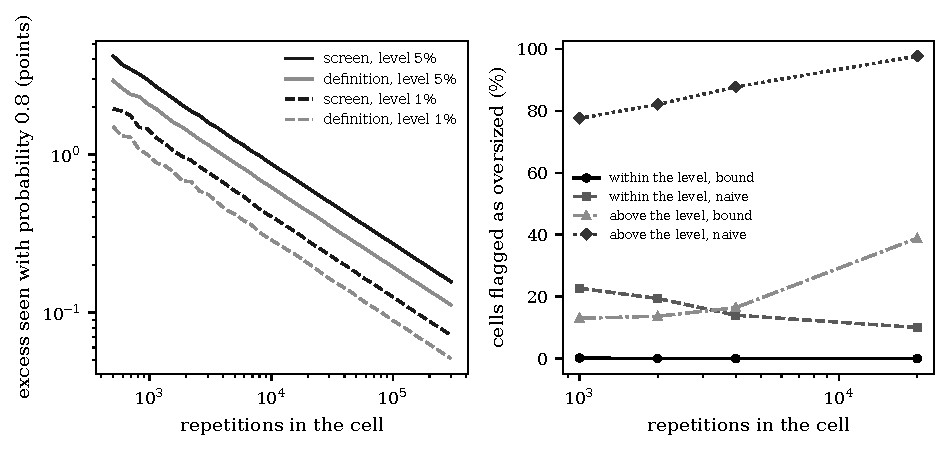
\includegraphics[width=\linewidth]{resolution}
\caption{Left: the excess over the level that the one-sided bound of the screen (black) and the Wilson interval of the definition (grey) detect with probability 0.8 against the number of repetitions of the cell, at the levels 5\% (solid) and 1\% (dashed); right: the share of cells flagged as oversized by the screen and by the naive rule among the tests within the level and among the tests above it.}
\label{fig:resolution}
\end{figure}

\subsection{The exact value beside the rate}
\label{sec:ab-exact}

The exact value does two things that the simulation alone cannot do.
It checks the generator: a generator whose probability of default is 5\,\% too high makes the binomial test reject \agMeanRateFive\,\% of the samples at the 5\,\% level instead of \binExactFive\,\%, which exceeds the bound of \boundFive\,\% and would read as an oversized test, when the defect is in the generator.
The agreement check of \eqref{eq:agree} flags that generator with probability \agFailFivePercent\,\% by exact calculation, and in \agSimFive\,\% of \agBlocks{} simulated blocks (\agSimTen\,\% for a probability of default 10\,\% too high), while it flags the correct generator in \agSimNone\,\% of the blocks, against the \agFailOne\,\% that the calculation gives.
A probability of default 2\,\% too high is flagged with probability \agFailTwoPercent\,\%: the check does not see errors of that size, and the limitations say so.
It also decides what the simulation cannot: the exact size of the Jeffreys test at 1\,\% is \jeffExactOne\,\%, above the level, and one cell of 4,000 repetitions flags an excess of that size with probability \jeffDetect\,\%.

\subsection{The number of repetitions}
\label{sec:ab-repetitions}

The number of repetitions sets the resolution.
\Cref{tab:resolution} gives the excess over the level that the bound sees with probability 0.8: \detFiveThousand{} points at 5\,\% for 1,000 repetitions, \detFiveFour{} for 4,000, \detFiveTwentyK{} for 20,000 and \detFiveTwoHundredK{} for 200,000, and \detOneThousand{}, \detOneFour{}, \detOneTwentyK{} and \detOneTwoHundredK{} points at 1\,\%.
The false flag probability of a test per cell is \flagThousand\,\% at 1,000 repetitions, \flagTest\,\% at 4,000 and \flagTwentyK\,\% at 20,000, so more repetitions buy resolution without costing specificity.
The cost is linear in the repetitions: the 200,000 repetitions per test of the replication, for the 21 tests, took \seedMinutes{} minutes on 24 worker processes.
Four thousand repetitions per size cell is a reasonable default for a first measurement, because it makes the standard error of a rate at 5\,\% about 0.3 points; it is not enough to certify a size, and the replication shows that a result of ``holds'' at 4,000 is a statement of no excess larger than about a point (\detIntFiveFour{} by the definition, \detFiveFour{} by the screen). A user who needs a size known to a tenth of a point must run 200,000 repetitions, and a user who needs only to exclude an excess of three points can run 1,000.
